Eine Cd-Lampe wird zwischen die Polschuhe eines Elektromagneten gebracht. Die Emissionslinien der Lampe werden durch mehrere Linsen transversal
zum Magnetfeld kollimiert und treffen anschließend auf ein Prisma, sodass sie nach der Wellenlänge aufgespaltet werden.

Mit einem Polarisationsfilter und einem Spalt kann der zu untersuchende Übergang nach Wellenlänge und Polarisation
ausgewählt werden. Anschließend wird das Spektrum auf eine Lummer-Gehrcke-Platte abgebildet, wodurch ein Interferenzmuster
entsteht.

Dieses wird mit einer Digitalkamera aufgenommen.

\begin{figure}
\centering
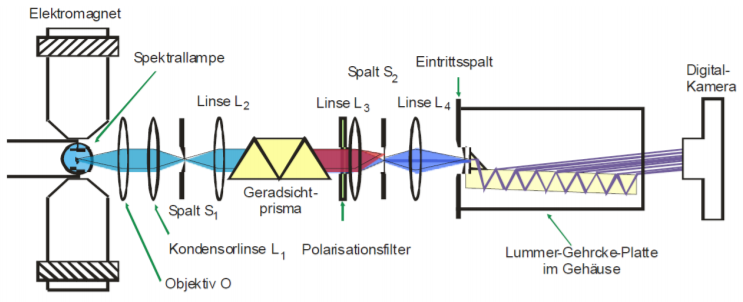
\includegraphics[width=\textwidth]{zeemanaufbau.png}
\caption{Schematischer Aufbau der Messapparatur \cite[2]{anleitung}.}
\label{fig:aufbau}
\end{figure}
